% Retrieval-augmented generation, and where it fails.
% ---------------------------------------------------------------------------
% style.tex --- shared preamble for every figure in book/figures/tikz/
%
% One style for all figures: Latin Modern, thin black lines, a light grey
% fill, and one accent colour used only to mark what is untrusted or wrong.
% Build with scripts/build_figures.sh; see book/figures/README.md.
% ---------------------------------------------------------------------------
\documentclass[tikz,border=6pt]{standalone}
\usepackage[T1]{fontenc}
\usepackage{lmodern}
\usetikzlibrary{arrows.meta,positioning,shapes.geometric,calc,fit,backgrounds}

\hyphenpenalty=10000   % short lines in boxes: ragged, never hyphenated

\definecolor{lightgrey}{gray}{0.92}
\definecolor{accent}{HTML}{9B2D20}

\tikzset{
  every picture/.style={
    line width=0.6pt,
    font=\small,
    >={Stealth[length=5pt,width=4pt]},
    node distance=14pt and 24pt,
  },
  % shapes
  box/.style={draw, rectangle, inner xsep=8pt, inner ysep=5pt,
              minimum height=22pt, align=center},
  grey/.style={box, fill=lightgrey},
  rounded/.style={box, rounded corners=9pt},
  decision/.style={draw, diamond, aspect=2.4, inner sep=1.5pt, align=center},
  group/.style={draw, dashed, rounded corners=5pt, inner sep=7pt},
  % text
  tag/.style={font=\footnotesize, align=center, inner sep=2pt},
  note/.style={font=\footnotesize\itshape, align=center, inner sep=2pt},
  code/.style={font=\small\ttfamily},
  codetag/.style={font=\footnotesize\ttfamily, align=center, inner sep=2pt},
  title/.style={font=\small\scshape, align=center, inner sep=2pt},
  % lines
  arrow/.style={->},
  back/.style={->, dashed},
  thin/.style={line width=0.4pt, gray},
  % the one accent, for what is untrusted, wrong or missing
  bad/.style={accent},
  badbox/.style={box, draw=accent, text=accent},
}

\begin{document}
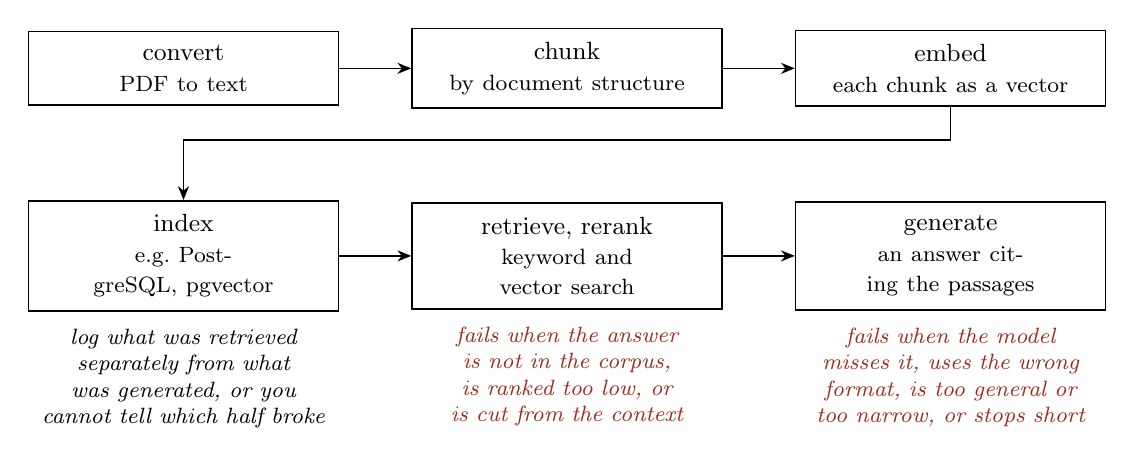
\begin{tikzpicture}[node distance=34pt and 26pt,
                    stage/.style={box, text width=96pt, align=center}]
  \node[stage] (convert) {convert\\ \footnotesize PDF to text};
  \node[stage, right=of convert] (chunk) {chunk\\ \footnotesize by document structure};
  \node[stage, right=of chunk] (embed) {embed\\ \footnotesize each chunk as a vector};
  \node[stage, below=of convert] (index) {index\\ \footnotesize e.g.\ PostgreSQL, pgvector};
  \node[stage, right=of index] (retrieve) {retrieve, rerank\\ \footnotesize keyword and vector search};
  \node[stage, right=of retrieve] (generate) {generate\\ \footnotesize an answer citing the passages};
  \draw[->] (convert) -- (chunk);
  \draw[->] (chunk) -- (embed);
  \draw[->] (embed.south) -- ++(0,-12pt) -| (index.north);
  \draw[->] (index) -- (retrieve);
  \draw[->] (retrieve) -- (generate);
  \node[note, below=4pt of retrieve, text width=104pt, text=accent]
    {fails when the answer is not in the corpus, is ranked too low, or is cut from the context};
  \node[note, below=4pt of generate, text width=104pt, text=accent]
    {fails when the model misses it, uses the wrong format, is too general or too narrow, or stops short};
  \node[note, below=4pt of index, text width=104pt]
    {log what was retrieved separately from what was generated, or you cannot tell which half broke};
\end{tikzpicture}
\end{document}
